\chapter{Data Acquisition}

\section{CAEN ADC DT5725S}

The first data-acquisition stage of the present NCAL commissioning campaign was based on a CAEN DT5725S desktop digitizer. In the public CAEN product documentation, the DT5725 and DT5725S are grouped into the same instrument class: an 8-channel, 14-bit, \SI{250}{MS/s} digitizer of the x725 family \citep{CAENDT5725Page}. After the Linux USB driver had been installed on the laboratory computer, a direct CAEN library probe identified the board used in this work as model \texttt{DT5725S}, with 8 channels and 14-bit conversion. The same probe also showed that the board was already configured with a DPP-PSD application firmware. For that reason, the first functional test was performed with \textit{CoMPASS}, rather than by immediately switching to a waveform-only workflow.

An important feature of the x725 platform is the use of a programmable FPGA rather than a single fixed acquisition logic. The same hardware can therefore be operated either as a waveform recorder or as a digital pulse processor, depending on the firmware image loaded onto the board \citep{CAENDT5725Page,CAENDWavePage}. This flexibility is highly relevant for detector-development work. If the main objective is to preserve the full sampled pulse for later offline analysis, then waveform recording is the natural mode. If, instead, the aim is online extraction of energy, timing, or pulse-shape observables with a smaller event size, then one of the DPP firmware families is generally more appropriate.

For practical operation, the \texttt{S} suffix must be treated carefully. CAEN presents the DT5725 and DT5725S together at product level, but the downloadable firmware packages are distributed separately for x725 and x725S devices. In that sense, the DT5725S should be understood as the \texttt{S}-series hardware revision of the same 8-channel \SI{250}{MS/s} digitizer platform: the overall DAQ role is unchanged, but the correct x725S firmware image must be used for upgrades or mode changes. This distinction is operationally important even when the high-level acquisition concept remains the same.

\subsection{Firmware families and operating modes}

The firmware choice determines what information is extracted online and how much data reduction is performed before storage. The main modes relevant to the DT5725S are summarized in Table~\ref{tab:dt5725s-firmware}. In the present commissioning, the installed firmware belongs to the DPP-PSD family, which is well aligned with fast first tests using scintillation detectors and PMT-like signals.

\begin{table}[htbp]
\centering
\caption{Firmware modes relevant to the DT5725S/x725S platform.}
\label{tab:dt5725s-firmware}
\small
\setlength{\tabcolsep}{5pt}
\renewcommand{\arraystretch}{1.08}
\begin{tabularx}{\textwidth}{>{\raggedright\arraybackslash}p{2.8cm}YY}
\toprule
Firmware & Main operating principle & Typical use case \\
\midrule
Waveform Recording (D-WAVE) & Oscilloscope-like waveform acquisition based on circular buffers, time-windowed recording, and dead-timeless multi-buffer management \citep{CAENDWavePage} & Detector R\&D, pulse-shape studies, charge integration, baseline studies, and flexible offline analysis of raw traces. \\
DPP-PHA & Digital replacement of a shaping amplifier plus peak-sensing ADC for pulse-height analysis \citep{CAENDPPPhaPage} & Gamma spectroscopy and precision energy measurements with HPGe, silicon detectors, or scintillators coupled to charge-sensitive front-end electronics. \\
DPP-PSD & Digital replacement of a dual-gate QDC, discriminator, and gate generator, with charge integration and pulse-shape discrimination \citep{CAENDPPPsdPage} & Scintillator readout, especially when neutron--gamma discrimination or fast timing is required. This is the firmware presently installed on the laboratory board. \\
DPP-DAW & Self-triggered acquisition with dynamic record length adjusted to the pulse duration, optimized for zero suppression and trigger-less operation \citep{CAENDPPDawPage} & Sparse-data systems, variable pulse lengths, and applications where efficient data reduction is important. \\
DPP-ZLEplus & Compressed waveform transfer with enhanced zero suppression and programmable look-back/look-forward windows around significant pulses \citep{CAENDPPZLEplusPage} & Acquisition scenarios where waveform fragments should be preserved, but the volume of baseline-only data must be reduced. \\
DPP-SUP & License bundle covering several DPP algorithms on a single supported digitizer \citep{CAENDPPSUPPage} & Convenient when the same hardware may need to switch between multiple DPP modes during development or deployment. \\
\bottomrule
\end{tabularx}
\end{table}

From a DAQ-design perspective, these firmware families correspond to different compromises between information content and throughput. Waveform recording maximizes retained information, because the full sampled trace is available for later analysis. The DPP modes instead move part of the signal processing into the FPGA and store higher-level observables such as integrated charge, pulse height, timing, or discrimination parameters. This reduces the event size and simplifies online monitoring, but it also couples the recorded data more strongly to the assumptions built into the chosen algorithm. For the first commissioning step, keeping the already installed DPP-PSD firmware was therefore the most conservative choice: it avoided an unnecessary firmware change while allowing immediate validation of the readout chain.

\subsection{Driver requirement on the acquisition computer}

For Linux-based operation, USB visibility at the operating-system level is not sufficient by itself. CAEN applications for Digitizer~1.0 boards rely on the CAEN software stack, including the communication and digitizer libraries used by programs such as WaveDump and CoMPASS \citep{CAENWaveDumpPage,CAENUSBDriverReadme2024}. In the present commissioning, the DT5725S was initially visible through the generic USB subsystem, but the CAEN libraries were still unable to open the device. Only after installation of the CAENUSBdrvB Linux driver did the expected device interface \texttt{/dev/usb/v1718\_0} appear; after that step, the same probe opened the board successfully and read back the model and firmware information.

This observation explains why the driver is mandatory on the acquisition computer. It does not merely provide user permissions for an already usable USB endpoint; rather, it supplies the device interface expected by the CAEN communication layer. In practical terms, the successful commissioning sequence on the laboratory PC was therefore: USB driver installation, verification of the \texttt{v1718} device node, successful low-level library access, and only then use of the graphical DAQ software.

\subsection{Software environment}

The DT5725S is embedded in a broader vendor software ecosystem, and different programs are appropriate for different firmware modes. The most relevant tools for the present work are summarized in Table~\ref{tab:dt5725s-software}.

\begin{table}[htbp]
\centering
\caption{Main software components relevant to the DT5725S.}
\label{tab:dt5725s-software}
\small
\setlength{\tabcolsep}{5pt}
\renewcommand{\arraystretch}{1.08}
\begin{tabularx}{\textwidth}{>{\raggedright\arraybackslash}p{2.8cm}YY}
\toprule
Software & Primary role & Relevance to the present setup \\
\midrule
CoMPASS & Multiparametric DAQ for CAEN DPP firmware, with simultaneous waveform, energy, timing, PSD, and list-mode handling \citep{CAENCoMPASSPage} & Natural front-end for the current DPP-PSD board configuration; used for the first successful functional test after driver installation. \\
WaveDump & Basic console readout program for boards running waveform-recording firmware; supports configuration files, rate readout, waveform display, and data export \citep{CAENWaveDumpPage} & Useful as a lightweight reference application and as an example of direct use of the CAEN libraries. It does not support DPP firmware. \\
WaveDump2 & Modern open-source GUI for waveform-recording operation, with oscilloscope-like plots, multi-board handling, configuration save/load, and ASCII or binary output \citep{CAENWaveDump2Page} & Most relevant if the DT5725S is later reflashed from DPP-PSD to x725S waveform-recording firmware for raw-trace studies. \\
CAEN Toolbox & Vendor utility for firmware upgrades, license management, PLL handling, and low-level board debugging \citep{CAENToolboxPage} & Relevant when changing firmware family, updating the board, or managing licenses during later stages of the DAQ campaign. \\
\bottomrule
\end{tabularx}
\end{table}

\paragraph{Practical launch commands.}
For Linux-based operation, the most useful user-level launch commands are straightforward. The DPP-oriented graphical front-end can be started as \texttt{CoMPASS}; if no shell launcher has been defined, the equivalent vendor-bundle invocation is \texttt{./CoMPASS} from the installation directory. The legacy console waveform reader is typically started as \texttt{WaveDump <configuration-file>}. The modern waveform GUI is started as \texttt{WaveDump2}, and the firmware and license-management utility is started as \texttt{caen-toolbox}. In practical use, the exact capitalization of these commands matters.

Two further remarks are important. First, the waveform-oriented tools are distinct from the DPP-oriented tools. The legacy WaveDump program and the more recent open-source WaveDump2 are intended for waveform-recording operation, whereas CoMPASS is designed around CAEN DPP algorithms \citep{CAENWaveDumpPage,CAENWaveDump2Page,CAENCoMPASSPage}. Second, CAEN also refers to CAENScope as a waveform-control environment in the waveform-recording documentation \citep{CAENDWavePage}; in the present work, however, the practically relevant distinction is between the current DPP-PSD plus CoMPASS path and a possible future x725S waveform-recording plus WaveDump2 path.

\subsection{Reproducible laboratory procedure}

To avoid repeating the same transport-layer debugging during later shifts, the first functional test should follow a fixed and documented sequence. On the present acquisition PC, the CAENUSBdrvB package was unpacked, built, and installed directly with \texttt{make} followed by \texttt{sudo make install}; this was the path actually used because a DKMS-based installation was not available on the host at that time. After installation, the decisive check was the appearance of the expected CAEN device node \texttt{/dev/usb/v1718\_0}.

For subsequent laboratory work, the minimum reproducible procedure is the following.

\begin{enumerate}
\item Verify that the digitizer is powered, connected by USB, and visible to the operating system as a CAEN device.
\item Confirm that the CAENUSBdrvB driver is installed for the running kernel and that the \texttt{v1718} device node is present.
\item Run a low-level CAEN access test, or an equivalent vendor utility, and verify that the board opens successfully and reports the expected model identifier \texttt{DT5725S}, channel count, and firmware information.
\item Start \textit{CoMPASS}, add the board as a direct USB connection with link number 0, and keep the board in its currently installed firmware family during the first validation step.
\item Enable one detector channel first, apply a conservative threshold and the correct signal polarity, and verify that both the trigger rate and the displayed waveform respond when a detector signal, source, or pulser is present.
\item Archive the accepted setup by saving the \textit{CoMPASS} configuration together with the date, serial number, firmware revision, driver package version, active channel list, and the location of the first validated data file.
\end{enumerate}

This sequence is intentionally modest, but it is sufficient to distinguish a solved infrastructure problem from a merely temporary success. A run should be treated as a valid commissioning reference only after the driver interface, low-level CAEN communication, graphical DAQ connection, and single-channel pulse response have all been demonstrated in the same session.

In summary, the present commissioning strategy was scientifically and technically motivated by the actual state of the hardware. The board already carried a DPP-PSD firmware, and the first bottleneck on the lab PC was not the firmware itself but the missing Linux USB driver. Once that driver was installed and the CAEN library stack could open the device, CoMPASS became the shortest path to a first validated acquisition. A later transition to full raw-waveform studies remains fully possible, but it would require loading the x725S waveform-recording firmware and switching to a waveform-oriented software stack.

\section{DOGMA analysis}
\label{subsec:dogma_analysis}

Once the front-end DAQ was validated, the central offline task was to transform the recorded DOGMA edge stream into a reusable set of cleaned pulses, timing observables, folded RF products, and final ROOT trees. In the present campaign, the active production workflow is kept in \path{Dogma_Analysis/Analysis/}, while exploratory or superseded utilities are moved to \path{Dogma_Analysis/Analysis/Archive/}. The workflow is edited locally in the mounted workspace, but the authoritative processing is executed remotely on \texttt{padiwa} against the canonical \path{/data6} filesystem. This split was adopted deliberately: it keeps the code under versioned local control while ensuring that large raw and refined datasets are processed where the storage and throughput are available.

\subsection{Execution model and data layout}

The present repository does not start from digitizer waveforms directly. Instead, it starts from DOGMA-produced raw edge files with names such as \texttt{NCAL\_...\_.dld.dat}. Upstream conversion to these files is external to the current analysis repository; the workflow described here begins once those files exist.

For reproducibility, the main storage layout is fixed.

\begin{itemize}
\item Raw DOGMA inputs are stored under
\path{/data6/Data/*.dld.dat}.
\item Cleaned pulse tables are stored under
\path{/data6/Data/Refined_Data/<run_key>_rawRefined/}.
\item Per-run analysis products are stored under
\path{/data6/Dogma_analysis_by_Dachi/Results/<run_key>/}.
\item Batch-comparison plots are collected under
\path{/data6/Dogma_analysis_by_Dachi/Results/Ch02_Position_Comparison/}.
\item Archived result sets are kept under
\path{/data6/Dogma_analysis_by_Dachi/Results/Archive/}
and archived cleaned-data directories under
\path{/data6/Data/Refined_Data/Archive/}.
\end{itemize}

The analysis uses a compact \emph{run key} derived from the raw filename, for example \path{NCAL_20us_Pos_3.4m_0000}. This run key is then used consistently for the refined directory, the result directory, the summaries, the ROOT outputs, and the comparison plots. This naming convention became important during repeated reruns, because it allowed regenerated products to be compared run by run rather than by full raw filename.

\subsection{From raw edges to cleaned pulses}

The first production step is implemented in \path{step01_dogma_raw_data_refiner.cpp} and driven by \path{step01_run_dogma_raw_data_refiner.py}. Its purpose is to convert raw edge information into a cleaned pulse table. Conceptually, the raw DOGMA file contains edge-level information, whereas most later physics studies require pulse-level quantities. The cleaner therefore performs the following tasks.

\begin{itemize}
\item It groups edges into trigger windows.
\item It matches rising and falling edges to form pulses with a well-defined rise time, fall time, and time-over-threshold (ToT).
\item It rejects isolated or inconsistent edges instead of silently promoting them to valid pulses.
\item It applies configurable acceptance limits, for example on allowed hit time and ToT.
\item It preserves run-level bookkeeping in a summary file so that anomalies are not hidden inside downstream histograms.
\end{itemize}

This step was essential for answering a basic but important conceptual question: whether the later ToT histograms could somehow be populated from unmatched or spurious edges. The conclusion of the cleaner study was that the production chain works at the pulse level. In other words, the downstream ToT observables are populated from accepted rise--fall pulse candidates, not from arbitrary isolated edges.

During development, special attention was paid to global-time discontinuities. The cleaner is also the natural place to guard against overlap after time resets, because this is the earliest point where trigger-window ordering and global timing information are available together. For that reason, the refined pulse table is treated as the canonical reusable intermediate product: once this file exists and has passed sanity checks, most later analysis stages can be regenerated without rereading the original raw edge file.

\subsection{Stage-wise derived products and code map}

After pulse cleaning, the current production chain proceeds through a sequence of step-numbered programs.

\begin{itemize}
\item Rates: analyzer \path{step02_dogma_cleaned_all_channel_rates.cpp}; runner \path{step02_run_cleaned_all_channel_rates.py}. These write cleaned-data rate products and summary tables.
\item Time-versus-ToT products: analyzer \path{step03_dogma_cleaned_all_channel_time_tot.cpp}; runner \path{step03_run_cleaned_all_channel_time_tot.py}. These write trigger-referenced and \texttt{ch0}-referenced time-versus-ToT products, plus per-channel ToT distributions.
\item RF recovery and folding: analyzer \path{step04_dogma_cleaned_all_channel_rf_period.cpp}; runner \path{step04_run_cleaned_all_channel_rf_period.py}. These write RF-period scans, folded phase profiles, and phase-versus-ToT maps.
\item \path{step01_write_cleaned_root_tree.py}: final \texttt{CleanedHits} ROOT export containing the pulse-level branches needed for later reuse.
\item \path{run_all_cleaned_analysis_chain.py}: the batch orchestrator that executes the full cleaned-data chain for all runs and collects comparison plots.
\item \path{phi_star_artifact_diagnostic.py}: a lightweight dedicated diagnostic added during the RF-artifact investigation to test whether diagonal structures are introduced by folding or are already present in the pre-fold observables.
\end{itemize}

For quick reference, Table~\ref{tab:dogma-analysis-workflow} condenses the active production chain into a compact workflow map.

\begin{table}[htbp]
\centering
\caption{Compact summary of the current DOGMA cleaned-data workflow.}
\label{tab:dogma-analysis-workflow}
\small
\setlength{\tabcolsep}{4pt}
\renewcommand{\arraystretch}{1.08}
\begin{tabularx}{\textwidth}{>{\raggedright\arraybackslash}p{1.1cm}>{\raggedright\arraybackslash}p{3.1cm}>{\raggedright\arraybackslash}p{3.8cm}X}
\toprule
Stage & Main code family & Primary output & Main role \\
\midrule
Input & DOGMA raw files & \path{*.dld.dat} & Upstream DOGMA edge stream used as the entry point to the present repository workflow. \\
01 & \path{step01_*} & Cleaned pulse TSV table & Rise--fall pairing, acceptance cuts, global-time sanity checks, and cleaned-pulse production. \\
02 & \path{step02_*} & Rate summaries and plots & All-channel cleaned-rate monitoring and run-level rate comparisons. \\
03 & \path{step03_*} & Trigger-ref and \texttt{ch0}-ref time-versus-ToT products & Per-channel timing structure, ToT spectra, and reference-channel validation. \\
04 & \path{step04_*} & RF scans, folded profiles, and phase-segment tables & RF period recovery, phase folding, and within-run phase-reset handling. \\
ROOT & \path{step01_write_cleaned_root_tree.py} & \texttt{CleanedHits} ROOT tree & Final reusable pulse-level export with RF annotations and run metadata. \\
Batch & \path{run_all_cleaned_analysis_chain.py} & Per-run result directories and comparison bundle & Reproducible multi-run execution of the full chain on the remote host. \\
\bottomrule
\end{tabularx}
\end{table}

The heavy numerical steps remain in compiled C++ code, while Python is used mainly for orchestration, file management, and rendering. This was an explicit efficiency choice. The current runners compile the active C++ analyzers with \texttt{g++ -std=c++17 -O2 -Wall -Wextra -pedantic}. In addition, the batch pipeline now reuses already compiled binaries when the source has not changed, so repeated full reruns do not waste time recompiling the cleaner and the rate analyzer for every run.

For the ToT-related observables, the current production defaults use \SI{1280}{} bins across a \SI{128}{ns} interval. The effective ToT bin width is therefore \SI{0.1}{ns}. This limit was adopted intentionally so that the text outputs, ROOT products, PNG figures, and PDF figures all remain consistent and sufficiently fine-grained for later physics cuts.

\subsection{Timing conventions and folded observables}

Two timing reference frames are used throughout the cleaned-data chain.

\begin{enumerate}
\item \textbf{Trigger-referenced time}, where pulse times are measured relative to the hardware trigger.
\item \textbf{Channel-0-referenced time}, where pulse times are measured relative to the accepted reference pulse on channel 0 within the same trigger window.
\end{enumerate}

The \texttt{ch0} reference is physically important because channel 0 carries the discriminated timing signal derived from the facility RF chain. In the current implementation, a \texttt{ch0} candidate is accepted only if its rise time and ToT fall inside a predefined validity window. If several valid candidates are present, the first valid one is selected, and companion statistics files are written so that this choice can be audited later.

For a non-reference channel, the key timing quantity is therefore
\begin{equation}
t_{\mathrm{ch0\,ref}} = t_{\mathrm{rise}}^{(\mathrm{ch})} - t_{\mathrm{rise}}^{(\mathrm{ch0})}.
\end{equation}

The RF-folding step then deduces a best RF period $P$ and a phase origin $\phi_0$ from a score channel, which is currently channel 2 by default. The folded phase is written using the \texttt{ch0}-referenced rise time,
\begin{equation}
\phi = \operatorname{mod}\!\left( t_{\mathrm{ch0\,ref}} - \phi_0,\; P \right).
\end{equation}

This distinction became important during debugging. Trigger-referenced times and channel-0-referenced times are both useful, but they do not answer the same physical question. In particular, the folded RF products are meant to characterize detector timing relative to the RF reference, so the physically correct phase coordinate is the channel-0-referenced one rather than the trigger-referenced one.

The final ROOT tree produced by \path{step01_write_cleaned_root_tree.py} stores the pulse-width branch \texttt{tot\_ns}, the trigger- and channel-0-referenced rise-time branches, and the RF annotation branches \texttt{rf\_phase\_ns} and \texttt{rf\_fold\_n}. In the current robust version, it also stores \texttt{rf\_segment\_id}, so later analyses can identify which within-run RF segment was used when the phase was assigned.

\subsection{Challenges encountered and how they were addressed}

Several conceptually different problems were encountered during commissioning. They are summarized here because the resulting solutions shape the present analysis design.

\paragraph{Edge pairing and channel-0 ambiguity.}
The first class of questions concerned whether the cleaner was pairing edges in a physically sensible way and how robust the \texttt{ch0} reference selection was when multiple candidates appeared in the same window. The response was twofold. First, the pulse cleaner was treated as the authoritative rise--fall pairing stage. Second, the runners were extended to write odd-\texttt{ch0} statistics and sample files, so ambiguous or rescued \texttt{ch0} selections could be inspected instead of inferred indirectly from final plots.

\paragraph{RF phase--ToT combs.}
The folded RF phase-versus-ToT plots showed persistent negative-slope diagonal structures, informally referred to during the work as zebra or comb patterns. A major conceptual question was whether these were created by the plotting and folding code itself or whether they reflected structure already present in the data. The decisive test used the dedicated diagnostic \path{phi_star_artifact_diagnostic.py}, together with direct comparisons between step-03 outputs and step-04 outputs. The conclusion was that the diagonal families are not a rendering artifact introduced by step 4. They are already present before RF folding and are therefore more likely to reflect preferred timing families in the upstream reference or signal chain.

This point is important for later readers: the step-04 folding code can sharpen or display these structures clearly, but it is not their primary origin.

\paragraph{Hardware interpretation of the comb structure.}
Once the software-side artifact hypothesis became unlikely, attention shifted to the hardware reference chain. In particular, the RF sine is converted to logic through a discriminator path, and the LeCroy 821 quad discriminator became a concrete suspect. The working interpretation is not that the discriminator necessarily destroys the data stream altogether, but that threshold-crossing families in the RF reference chain can create structured timing bunching. In that scenario, the software is correctly exposing a reference-chain feature rather than inventing it.

\paragraph{Cyclotron off/on phase resets within a run.}
An additional challenge was the possibility that the cyclotron could be stopped and restarted during a single run. Under that condition, one run-level phase origin is no longer sufficient: early and late parts of the run can carry different RF offsets. The original implementation of step 4 used a single phase origin for the full run, and the final ROOT writer then reused that same single solution. This was identified as a real robustness problem.

The current solution is a segment-aware phase guard. The patched step-4 analyzer now searches the score pulses in time-ordered blocks, looks for persistent phase jumps rather than one-off fluctuations, and writes a segment table in \path{RF_period_scan/*_phase_segments.tsv}. The RF summary records whether the run was treated in global or segmented mode, and the final ROOT writer consumes the same segment information when filling \texttt{rf\_phase\_ns}, \texttt{rf\_fold\_n}, and \texttt{rf\_segment\_id}. Conceptually, this means that a within-run restart no longer forces the full run to share one RF phase origin.

\paragraph{Cost of reruns.}
The batch studies also showed that a rerun is not dominated solely by the initial cleaner. For the large runs, the RF-folding stage and the final ROOT export can each consume several hours. This observation motivated two design choices. First, restart handling was implemented without invalidating the cleaned pulse tables, so the expensive edge-cleaning stage does not need to be repeated just to improve RF segmentation. Second, compilation reuse was enabled for repeated batch executions. The workflow therefore remains quality-first, but it avoids unnecessary rebuild overhead.

\subsection{Reusability and batch production}

The batch interface for the current production chain is \path{run_all_cleaned_analysis_chain.py}. For each raw input file, it performs cleaning, rates, time-versus-ToT, RF folding, final cleaned ROOT writing, and collection of channel-2 comparison plots. The resulting comparison bundle is intended to make run-by-run inspection practical after long remote productions.

Several conventions were adopted specifically for long remote campaigns.

\begin{itemize}
\item Large result files are kept remote on \texttt{padiwa}; only small summaries and selected artifacts should be mirrored locally unless there is a specific reason to do otherwise.
\item Previous result sets are archived rather than overwritten when a major production rerun is launched.
\item The cleaned pulse table is treated as the stable handoff between raw edge decoding and higher-level timing analysis.
\item Heavy transformations remain in C++, while Python wrappers provide orchestration and output management.
\item Full-run batch processing is kept sequential by default, because disk I/O and ROOT writing are already heavy; aggressive multi-run parallelism was judged less robust than a controlled single-run pipeline on the current remote host.
\end{itemize}

In its current form, the DOGMA chain should be regarded as the robust production baseline for the commissioning data set. It already incorporates solutions to the most consequential analysis-side problems encountered so far: pulse-level cleaning, explicit \texttt{ch0} auditing, consistent time-versus-ToT products, dedicated RF diagnostics, and segment-aware handling of within-run RF phase resets. At the time of writing, the full remote rerun with this patched version is in progress and therefore serves as the definitive end-to-end validation of the present design.

\subsection{Background treatment and gamma--neutron timing reference}

The folded RF phase-versus-ToT plots are useful for developing gamma--neutron separation strategies, but they should not be interpreted as direct particle-identification maps without a background model. The radiation field seen by NCAL is mixed. It can contain prompt gammas from source-station materials, secondary capture gammas in hydrogenous material, room and shielding backgrounds, scattered neutrons, continuum neutrons from the beryllium target, random coincidences, electronic pickup, and residual artifacts from the timing-reference chain. For this reason, a compact region in phase--ToT space should be called gamma-like or neutron-like only after the non-beam and off-region contributions have been characterized.

The working strategy is therefore hierarchical. First, beam-off, no-target, blocked-aperture, or sideband regions should be used where available to estimate components that are not correlated with the prompt beam timing. Second, cleanly separated regions of the position scan can be used to define empirical gamma-like and neutron-like templates. Third, regions where the two populations overlap should be treated statistically rather than by hard event labels. In an overlapped phase--ToT region, the observed density should be represented schematically as
\begin{equation}
N(\phi,\mathrm{ToT}) = A_{\gamma}G(\phi,\mathrm{ToT}) + A_{n}N_{n}(\phi,\mathrm{ToT}) + B(\phi,\mathrm{ToT}),
\end{equation}
where \(G\) is the prompt-gamma-like template, \(N_{n}\) is the neutron-like template, and \(B\) is the residual background model. Under such conditions, individual hits cannot be assigned uniquely to gamma or neutron populations using phase and ToT alone. They should instead receive probabilistic weights or be used only in fitted yield estimates with an explicit overlap uncertainty.

An analytical time-of-flight reference is still needed to show why the position scan is expected to help. For a detector-face distance \(d\), the prompt-gamma time is
\begin{equation}
t_{\gamma}(d) = \frac{d}{c},
\end{equation}
while a neutron with kinetic energy \(E_{n}\) has
\begin{equation}
\beta_{n}(E_{n}) = \sqrt{1 - \left(1 + \frac{E_{n}}{m_{n}c^{2}}\right)^{-2}},
\qquad
t_{n}(d,E_{n}) = \frac{d}{\beta_{n}c}.
\end{equation}
The reference separation is therefore
\begin{equation}
\Delta t(d,E_{n}) = t_{n}(d,E_{n}) - t_{\gamma}(d).
\end{equation}
For the present campaign, \SI{30}{MeV} is used as the main reference energy because the reviewed \(p+\mathrm{Be}\) literature places the prominent high-energy forward-neutron structure near \SIrange{30}{32}{MeV}, with the thick-target spectrum extending up to about \SI{33}{MeV}. This should be understood as a reference curve for fast neutrons, not as a complete source-spectrum model.

Figure~\ref{fig:gamma-neutron-tof-reference-positions} shows the resulting prompt-gamma and fast-neutron time-of-flight curves for the position-scan distances. The \SI{30}{MeV} reference gives separations of about \SI{28.5}{ns}, \SI{34.6}{ns}, \SI{40.7}{ns}, \SI{50.9}{ns}, \SI{59.0}{ns}, and \SI{67.2}{ns} at \SIlist{2.8;3.4;4.0;5.0;5.8;6.6}{m}, respectively. Since slower continuum neutrons arrive later, this reference marks the early fast-neutron scale rather than the full neutron timing envelope.

\begin{figure}[htbp]
\centering
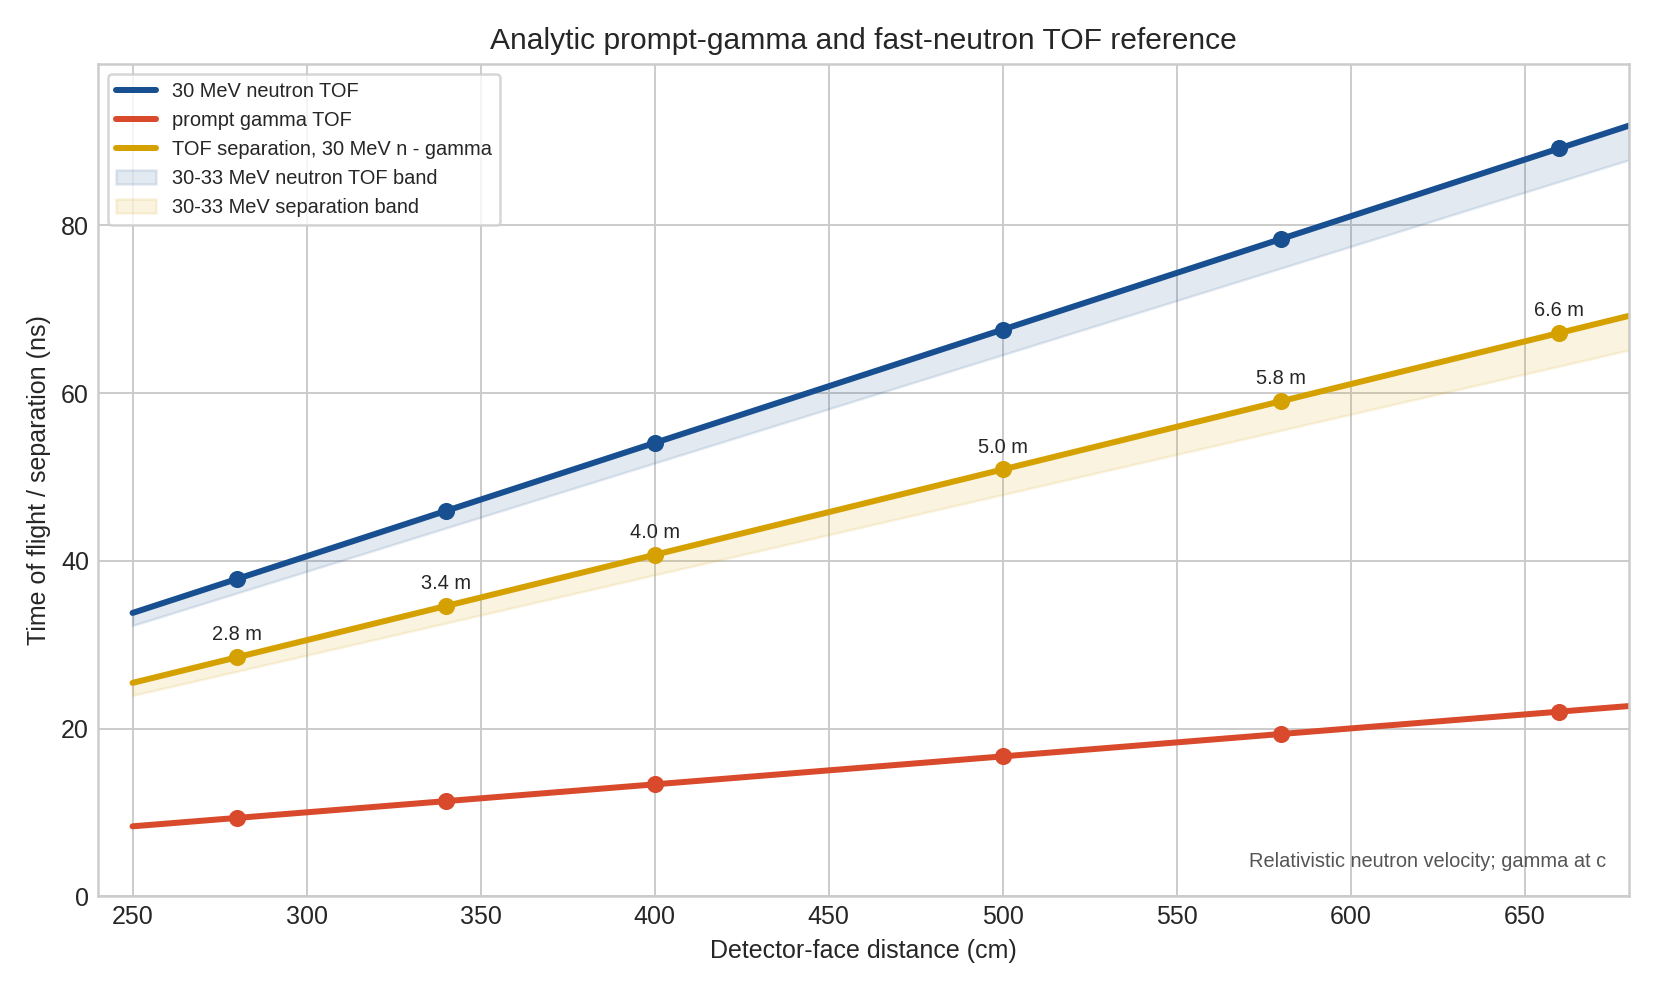
\includegraphics[width=0.92\textwidth]{figures/Gamma_Neutron_deltaTOF_30MeV_reference_positions.png}
\caption{Analytical prompt-gamma and fast-neutron time-of-flight reference for the NCAL position scan. The central neutron curve uses \SI{30}{MeV}; the shaded band indicates the small change between \SI{30}{MeV} and \SI{33}{MeV}. The \SI{30}{MeV} choice is a representative fast-neutron reference within the high-energy part of the \SI{35}{MeV} proton-on-beryllium spectrum, not a monoenergetic source assumption.}
\label{fig:gamma-neutron-tof-reference-positions}
\end{figure}

The qualitative motivation for this treatment is visible directly in the folded RF phase-versus-ToT products. Figure~\ref{fig:position-scan-phase-tot-panel} collects representative channel-2 maps from the completed position-scan runs, with the detector-face distance stated explicitly above each panel. The compact prompt-like island remains narrow in phase and ToT, while the broader neutron-dominated structure changes its relative timing as the detector distance is varied. The figure is included to show the observable space in which the later template or mixture analysis must operate; the different panels should not be read as an absolute yield comparison because the displayed density scales are plot-level renderings.

\begin{landscape}
\begin{figure}[p]
\centering
\begin{minipage}{0.32\linewidth}
\centering
{\small\bfseries Detector face: \SI{2.8}{m}}\\[0.25em]
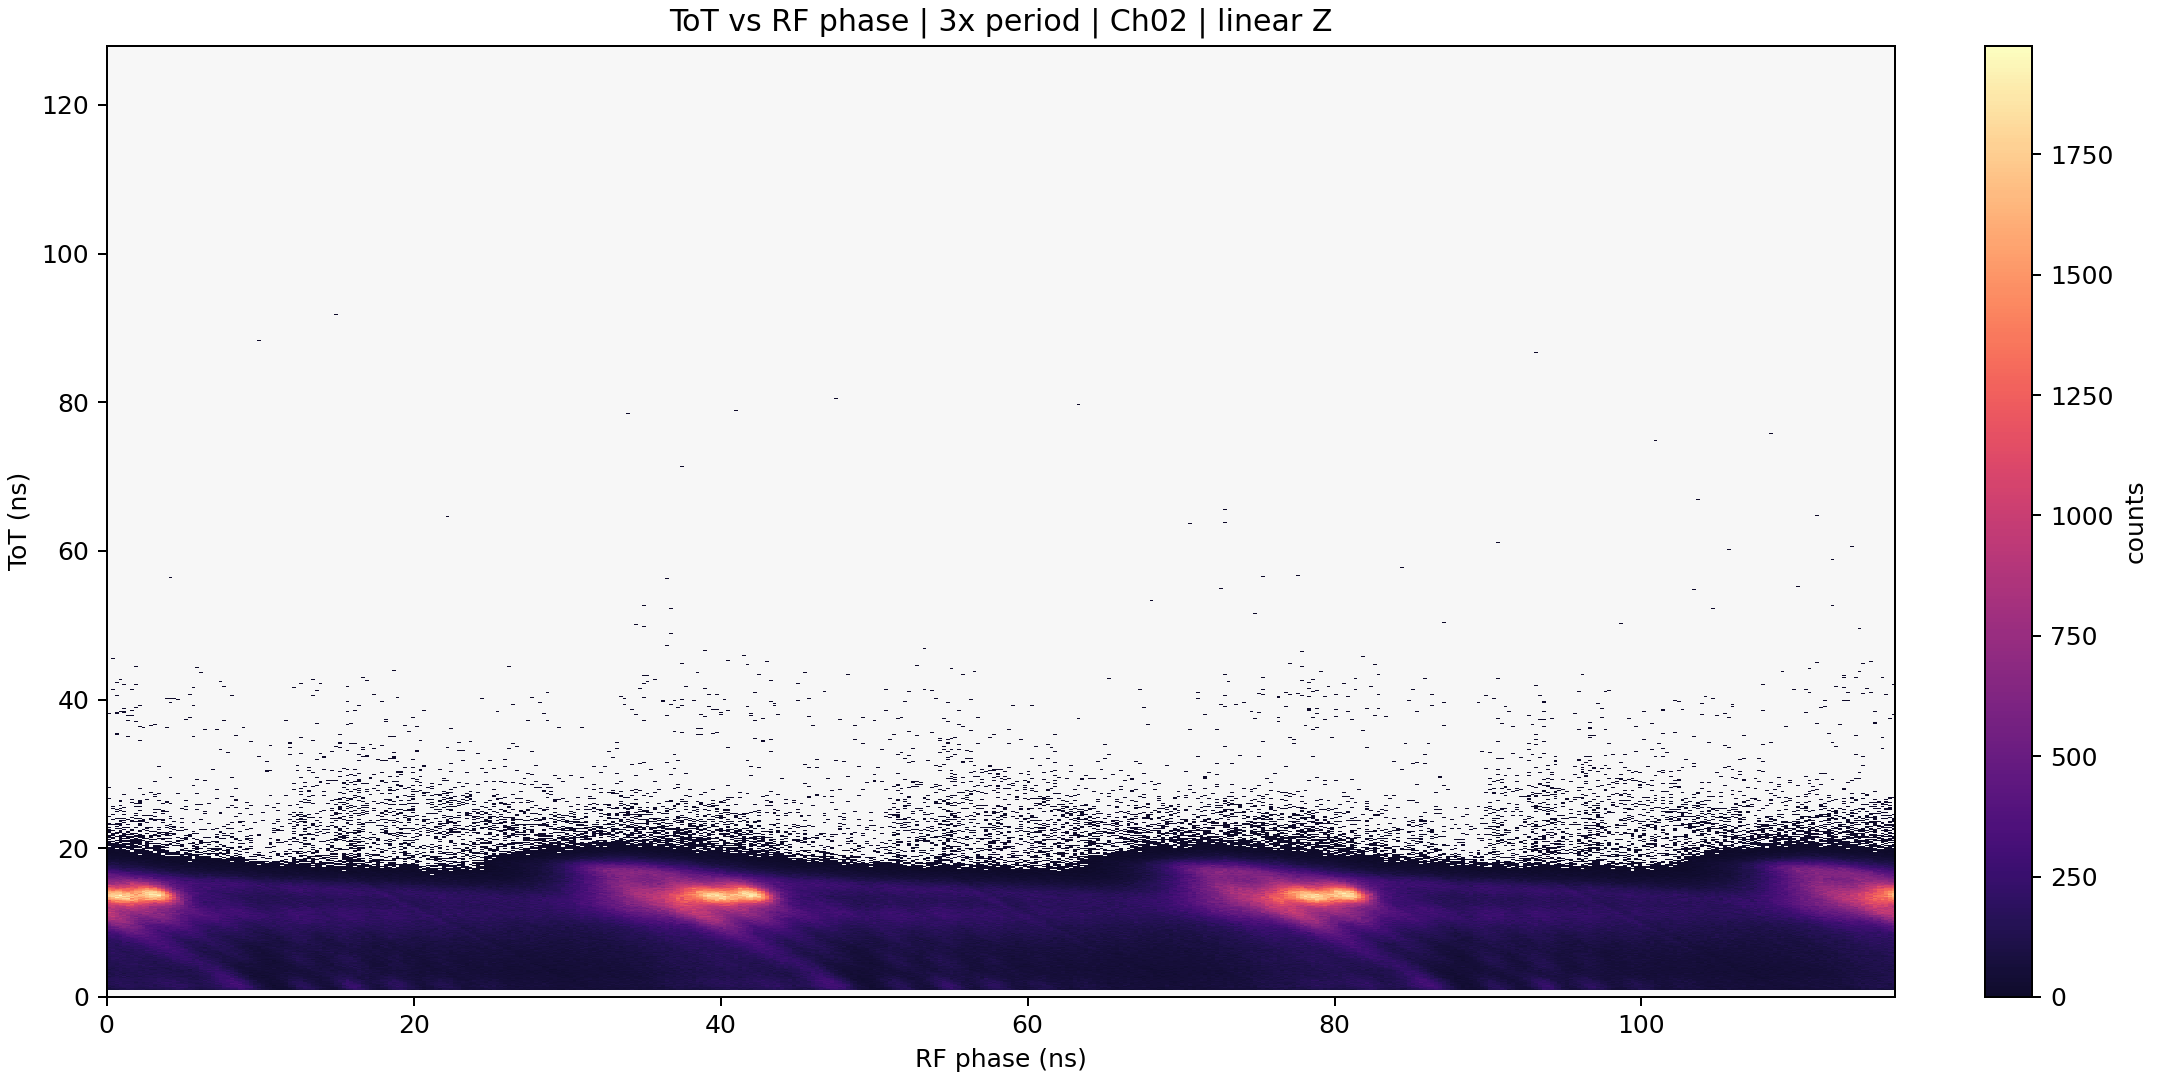
\includegraphics[width=\linewidth]{figures/phase_tot_position_scan/pos_2p8m_ch02_rf_phase_3x_vs_tot.png}
\end{minipage}\hfill
\begin{minipage}{0.32\linewidth}
\centering
{\small\bfseries Detector face: \SI{3.4}{m}}\\[0.25em]
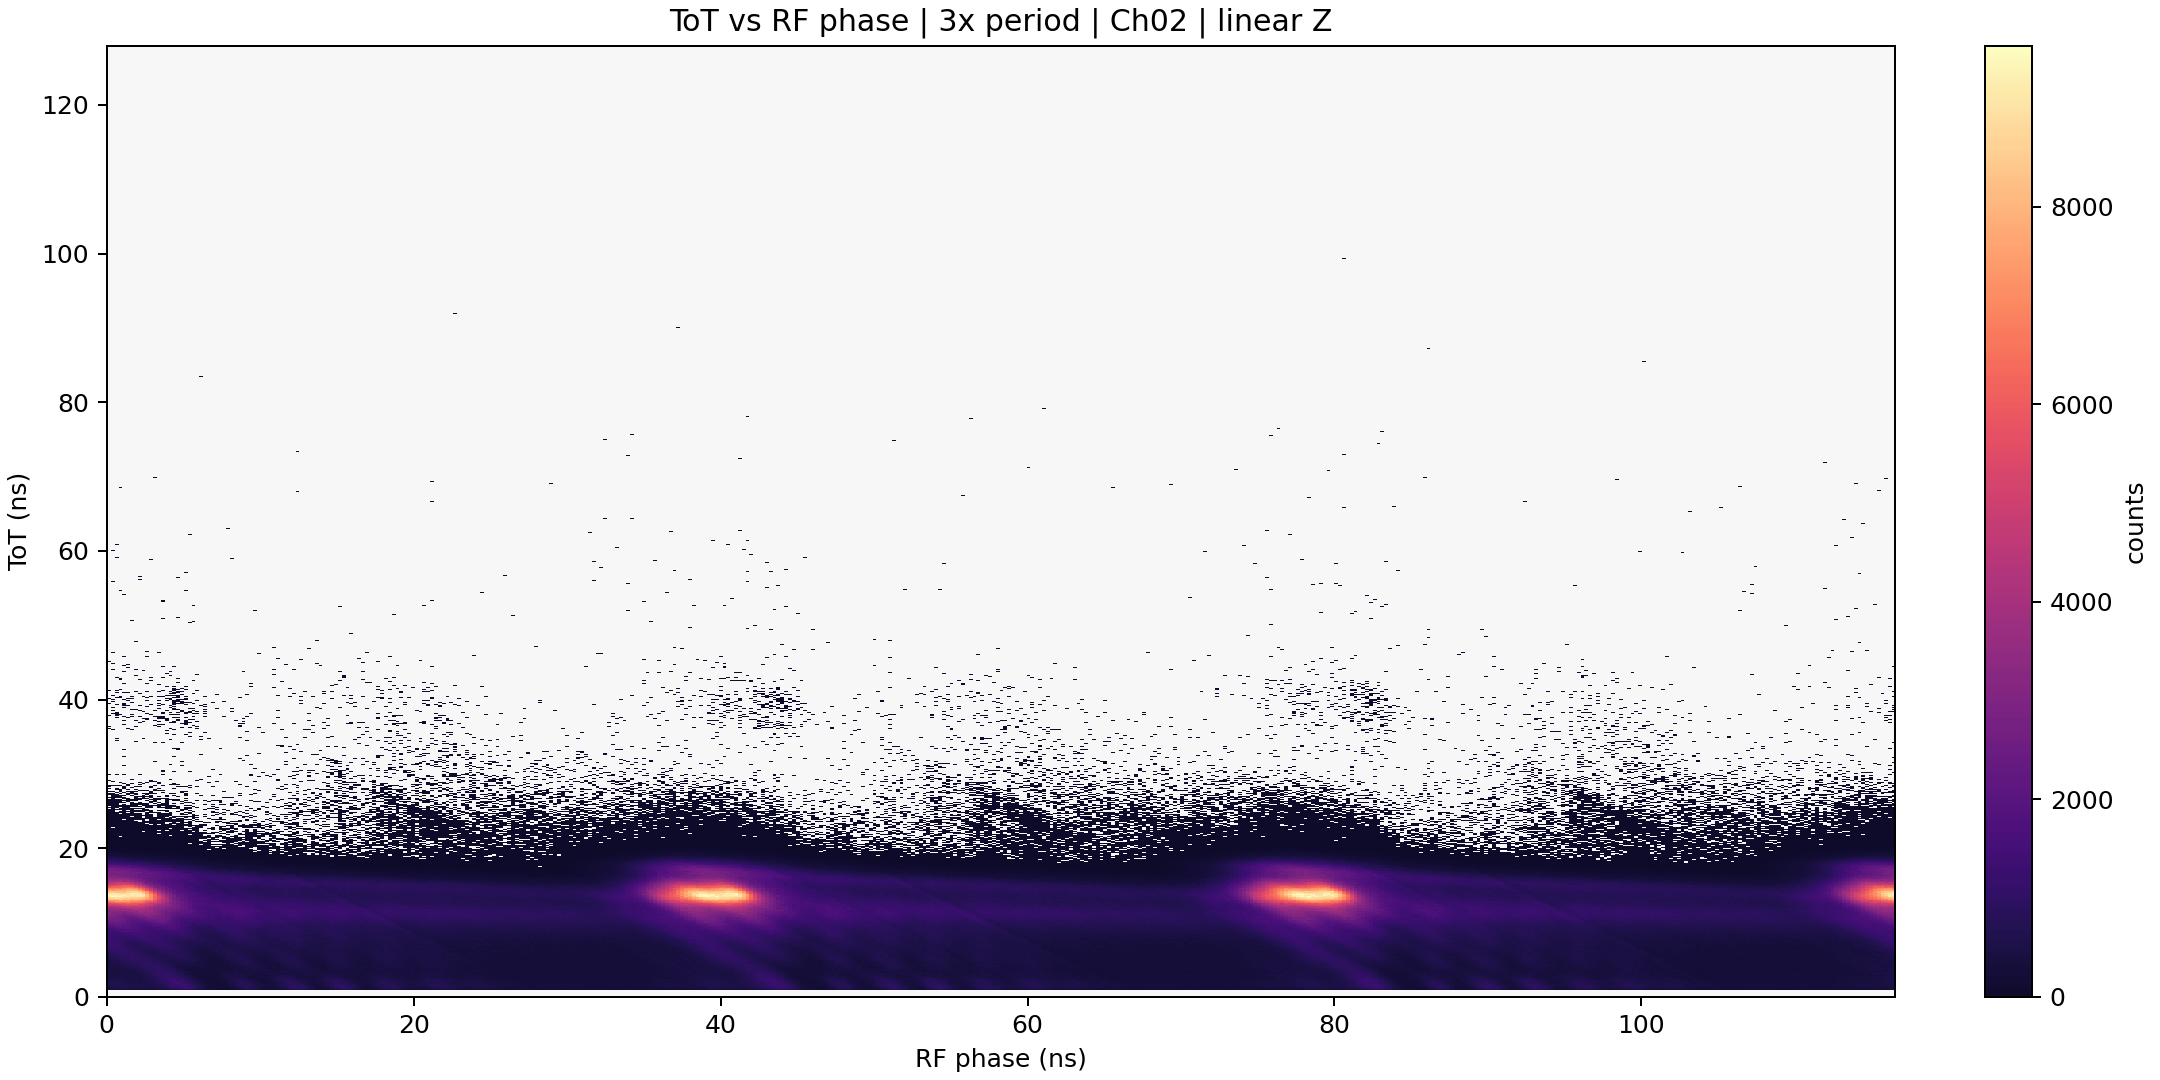
\includegraphics[width=\linewidth]{figures/phase_tot_position_scan/pos_3p4m_ch02_rf_phase_3x_vs_tot.png}
\end{minipage}\hfill
\begin{minipage}{0.32\linewidth}
\centering
{\small\bfseries Detector face: \SI{4.0}{m}}\\[0.25em]
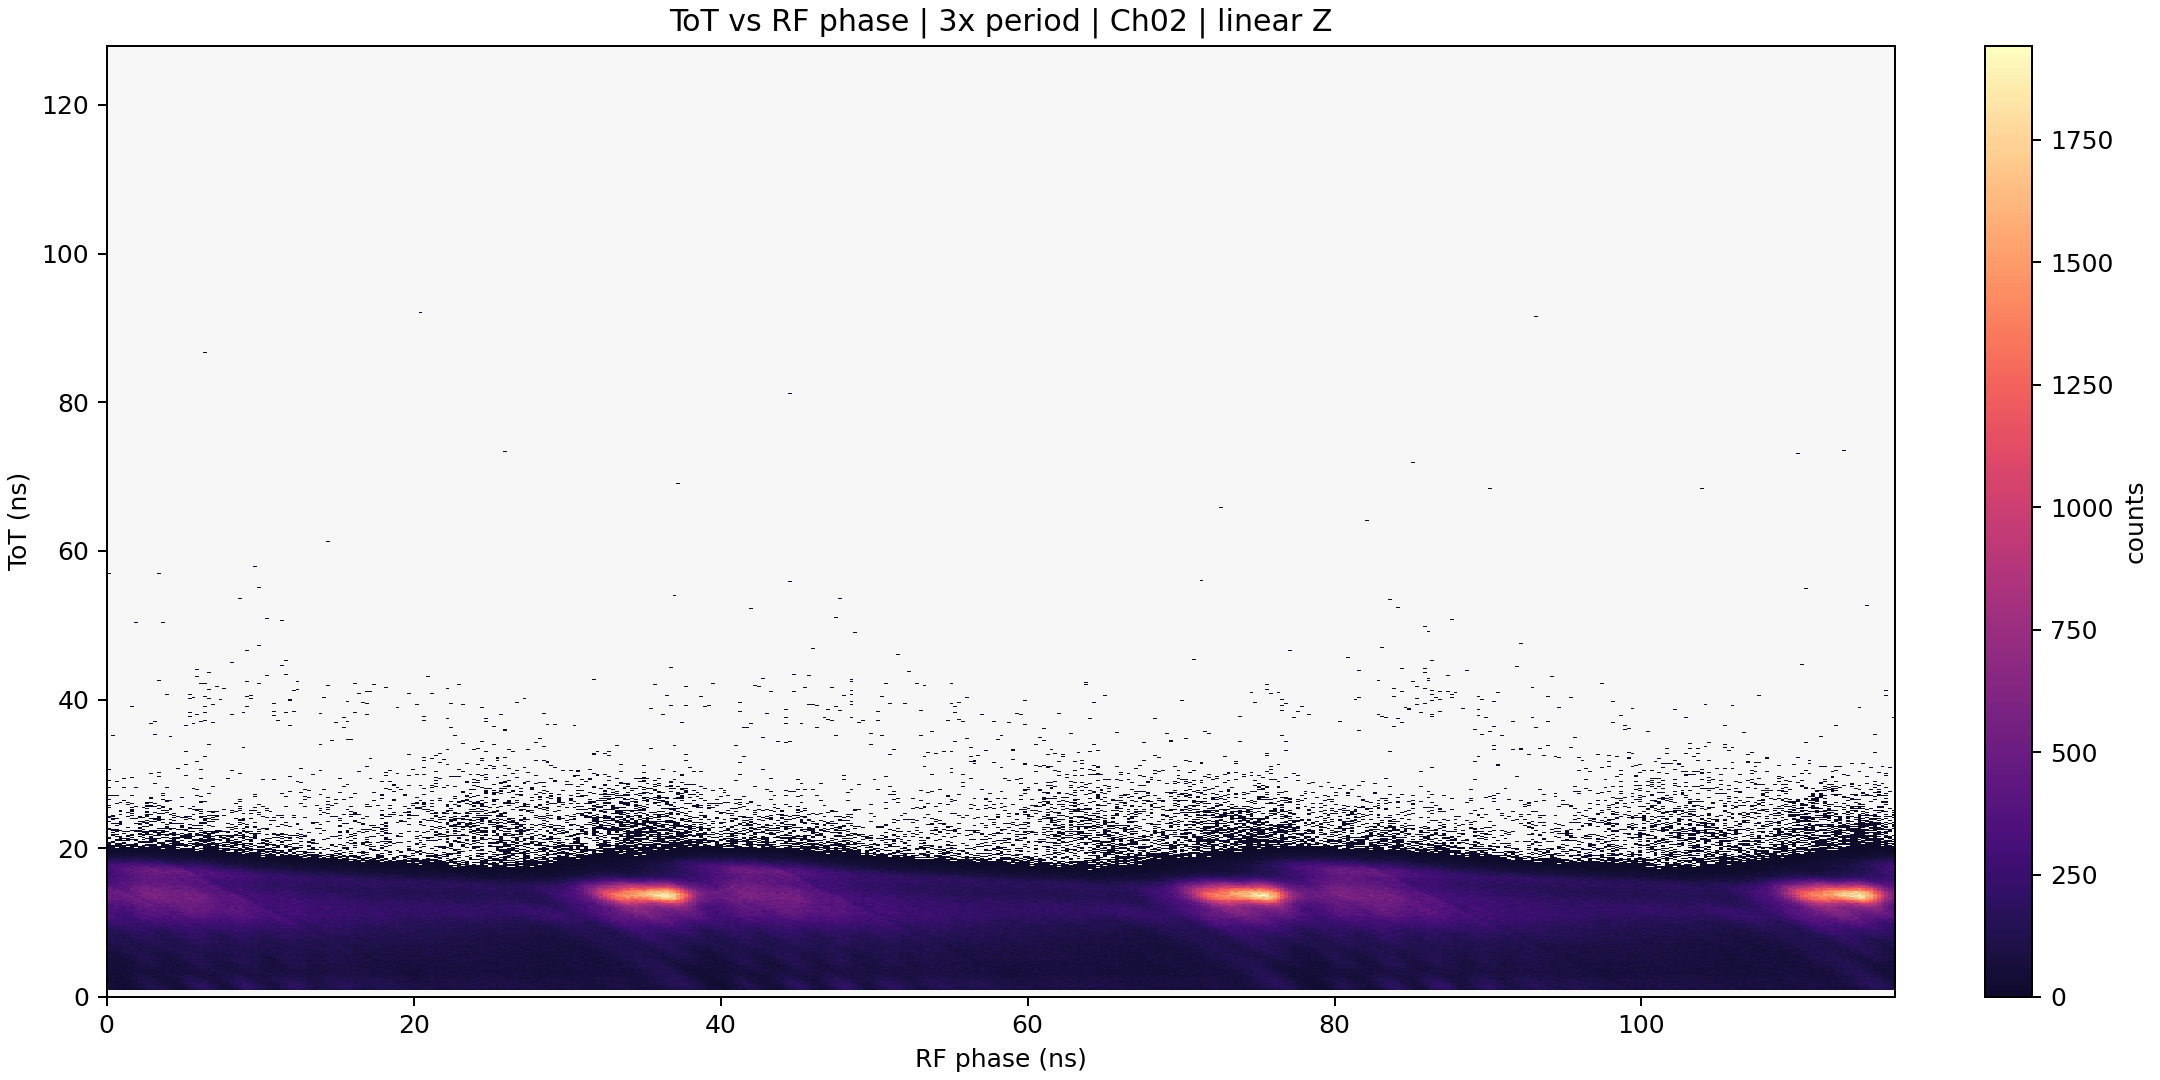
\includegraphics[width=\linewidth]{figures/phase_tot_position_scan/pos_4p0m_ch02_rf_phase_3x_vs_tot.png}
\end{minipage}

\vspace{0.5cm}

\begin{minipage}{0.32\linewidth}
\centering
{\small\bfseries Detector face: \SI{5.0}{m}}\\[0.25em]
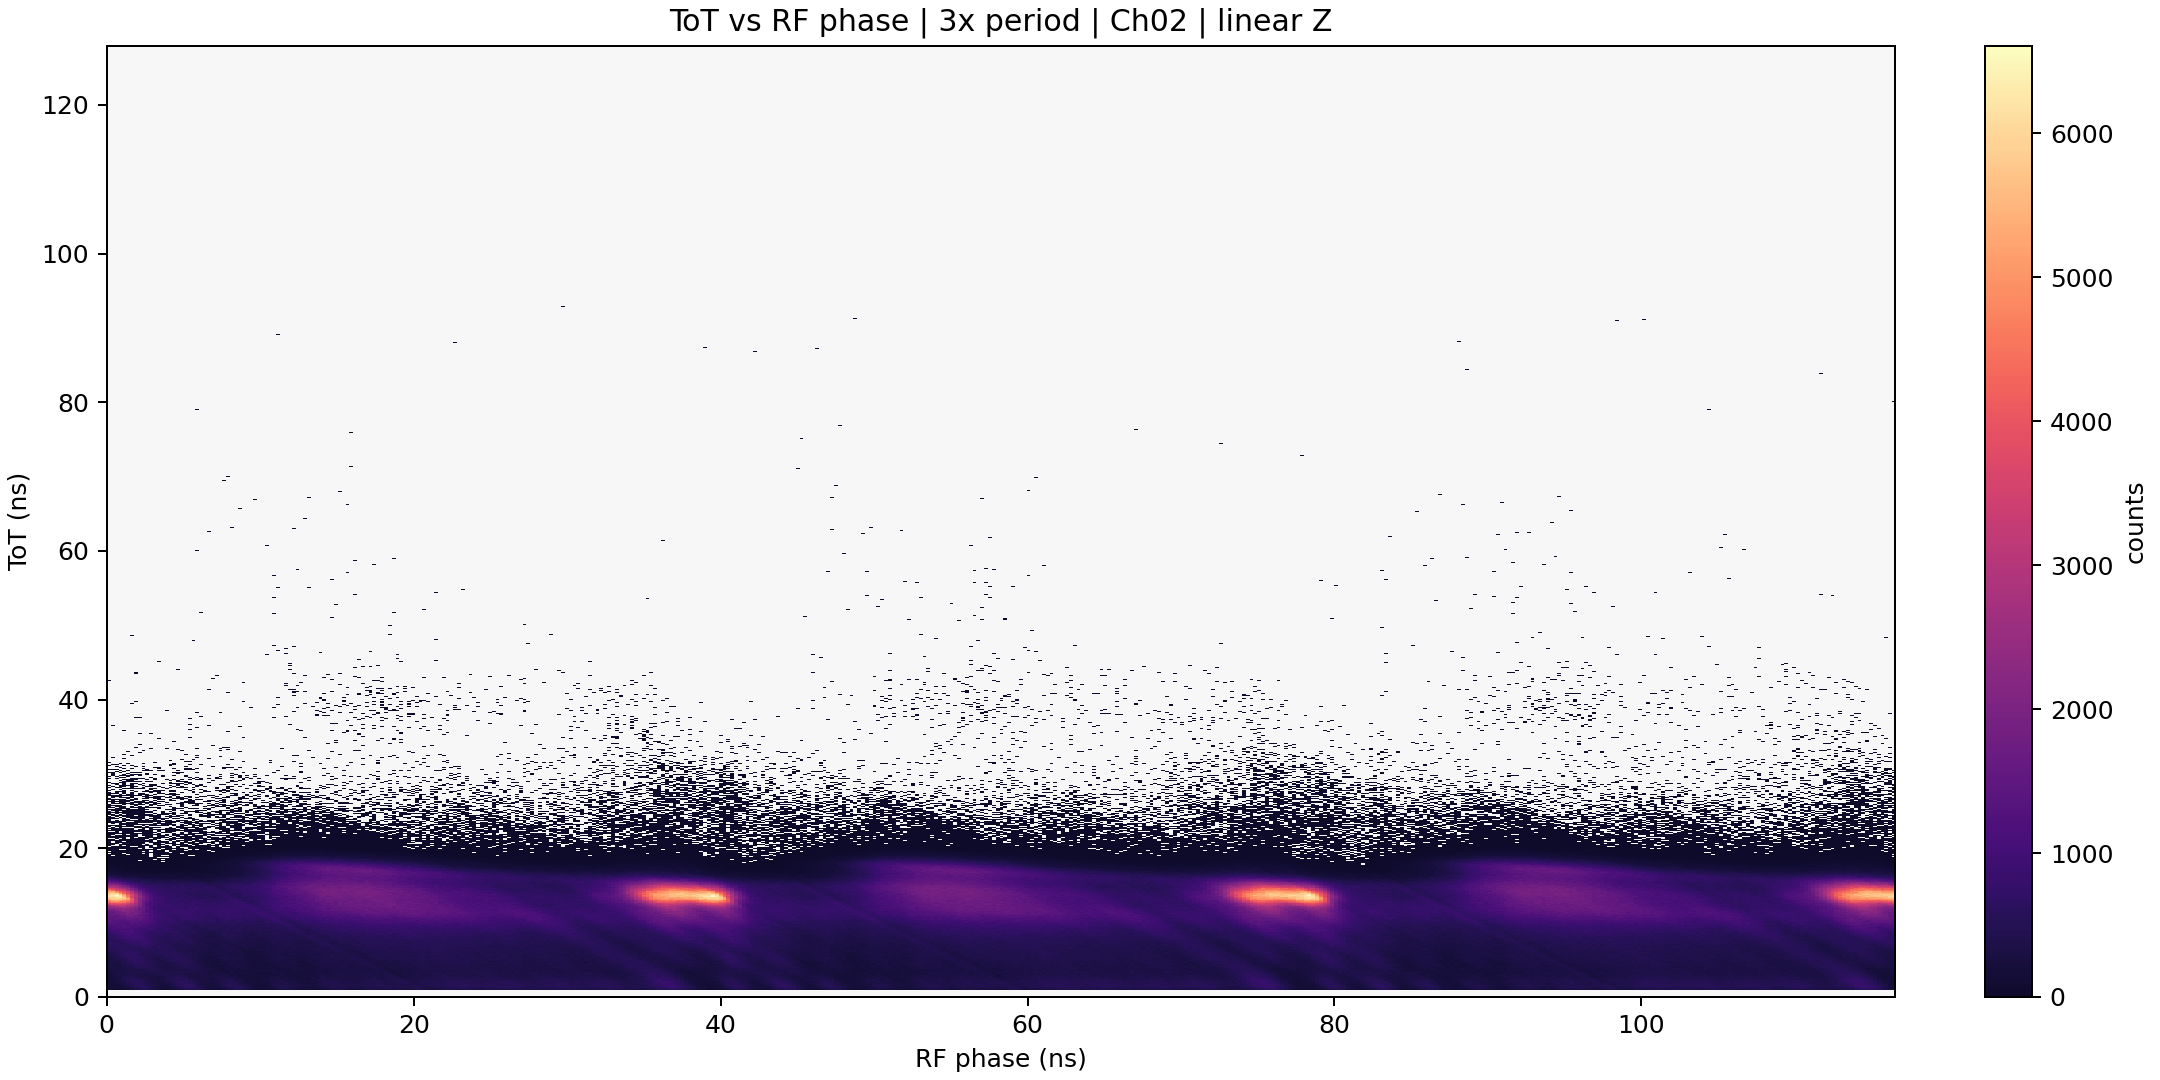
\includegraphics[width=\linewidth]{figures/phase_tot_position_scan/pos_5p0m_ch02_rf_phase_3x_vs_tot.png}
\end{minipage}\hfill
\begin{minipage}{0.32\linewidth}
\centering
{\small\bfseries Detector face: \SI{5.8}{m}}\\[0.25em]
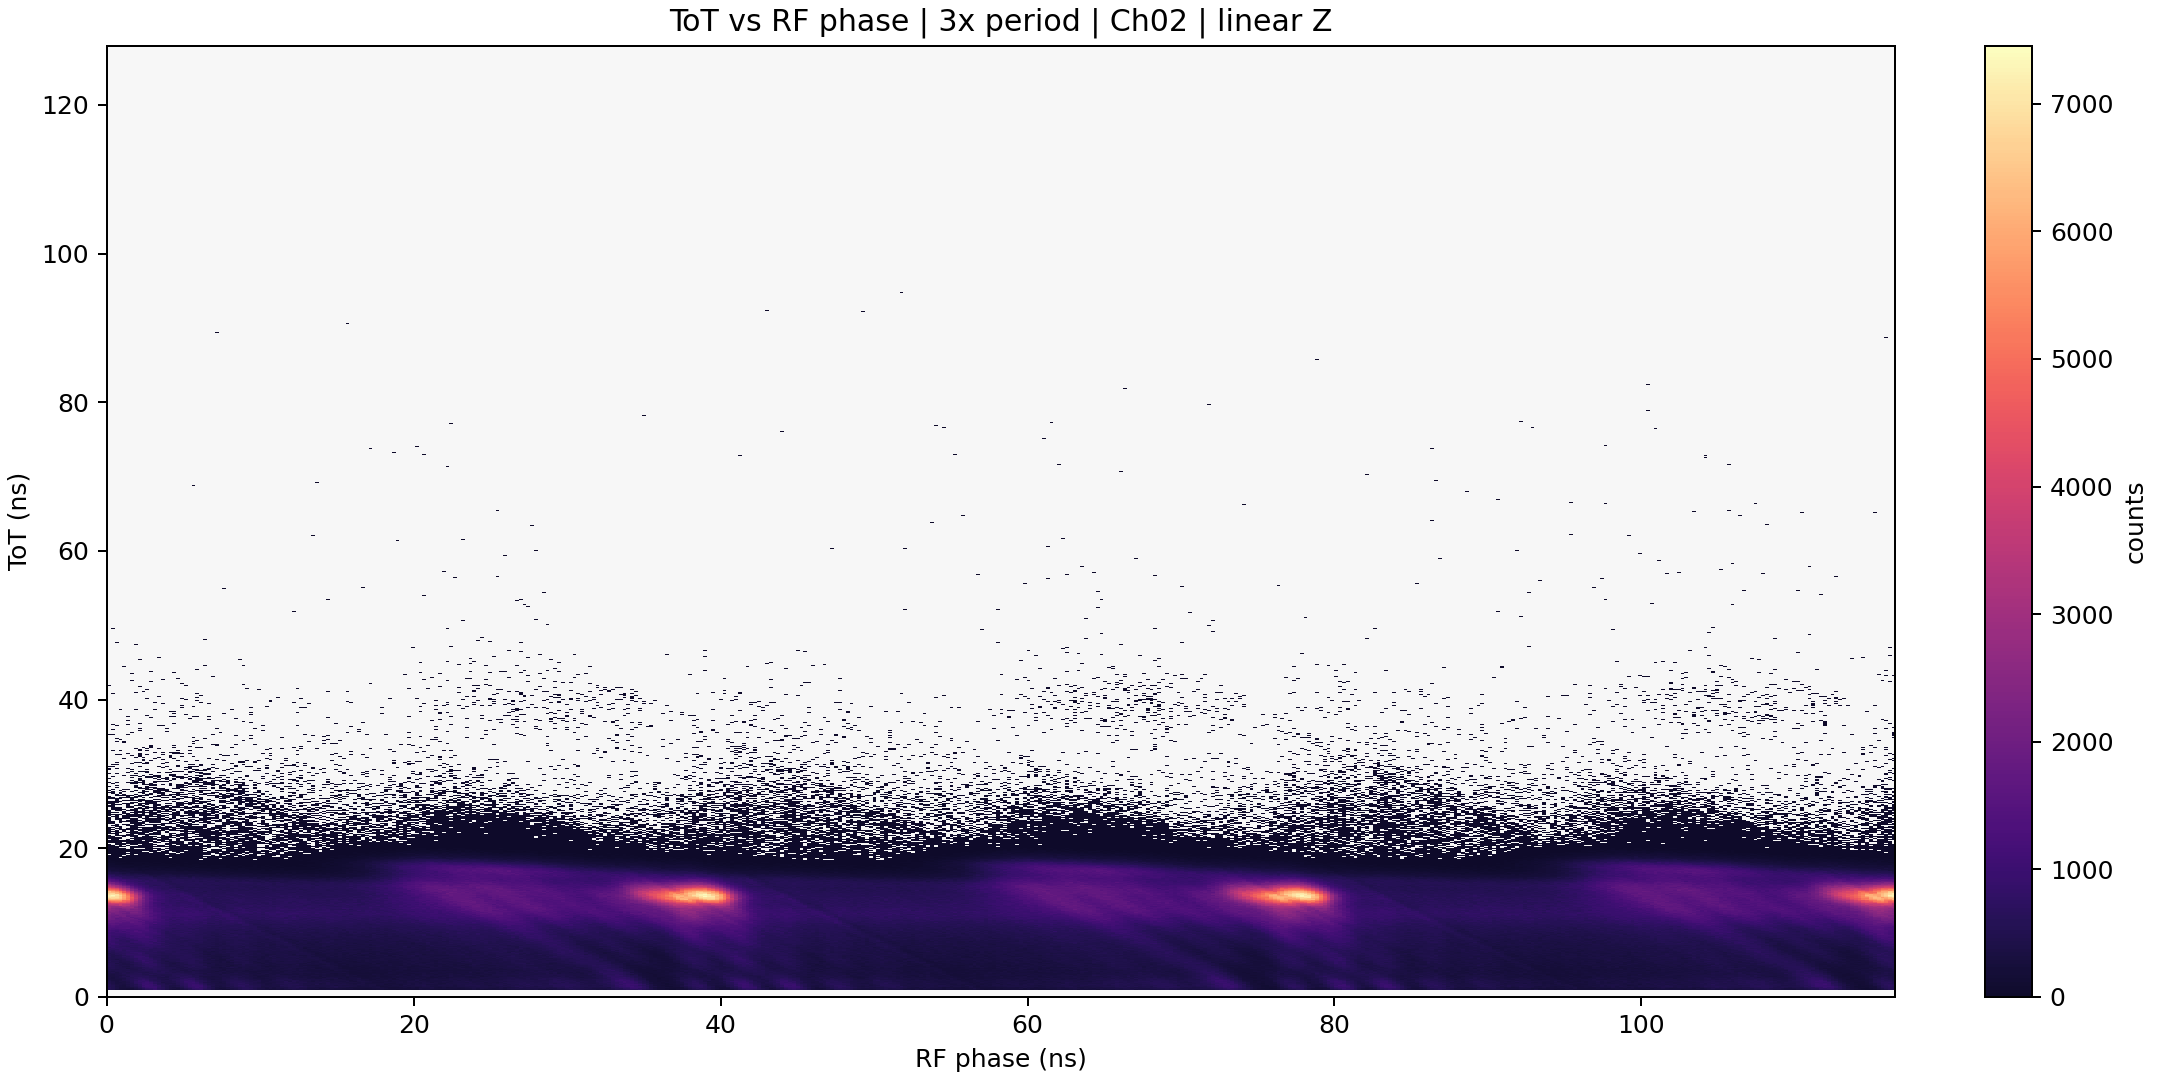
\includegraphics[width=\linewidth]{figures/phase_tot_position_scan/pos_5p8m_ch02_rf_phase_3x_vs_tot.png}
\end{minipage}\hfill
\begin{minipage}{0.32\linewidth}
\centering
{\small\bfseries Detector face: \SI{6.6}{m}}\\[0.25em]
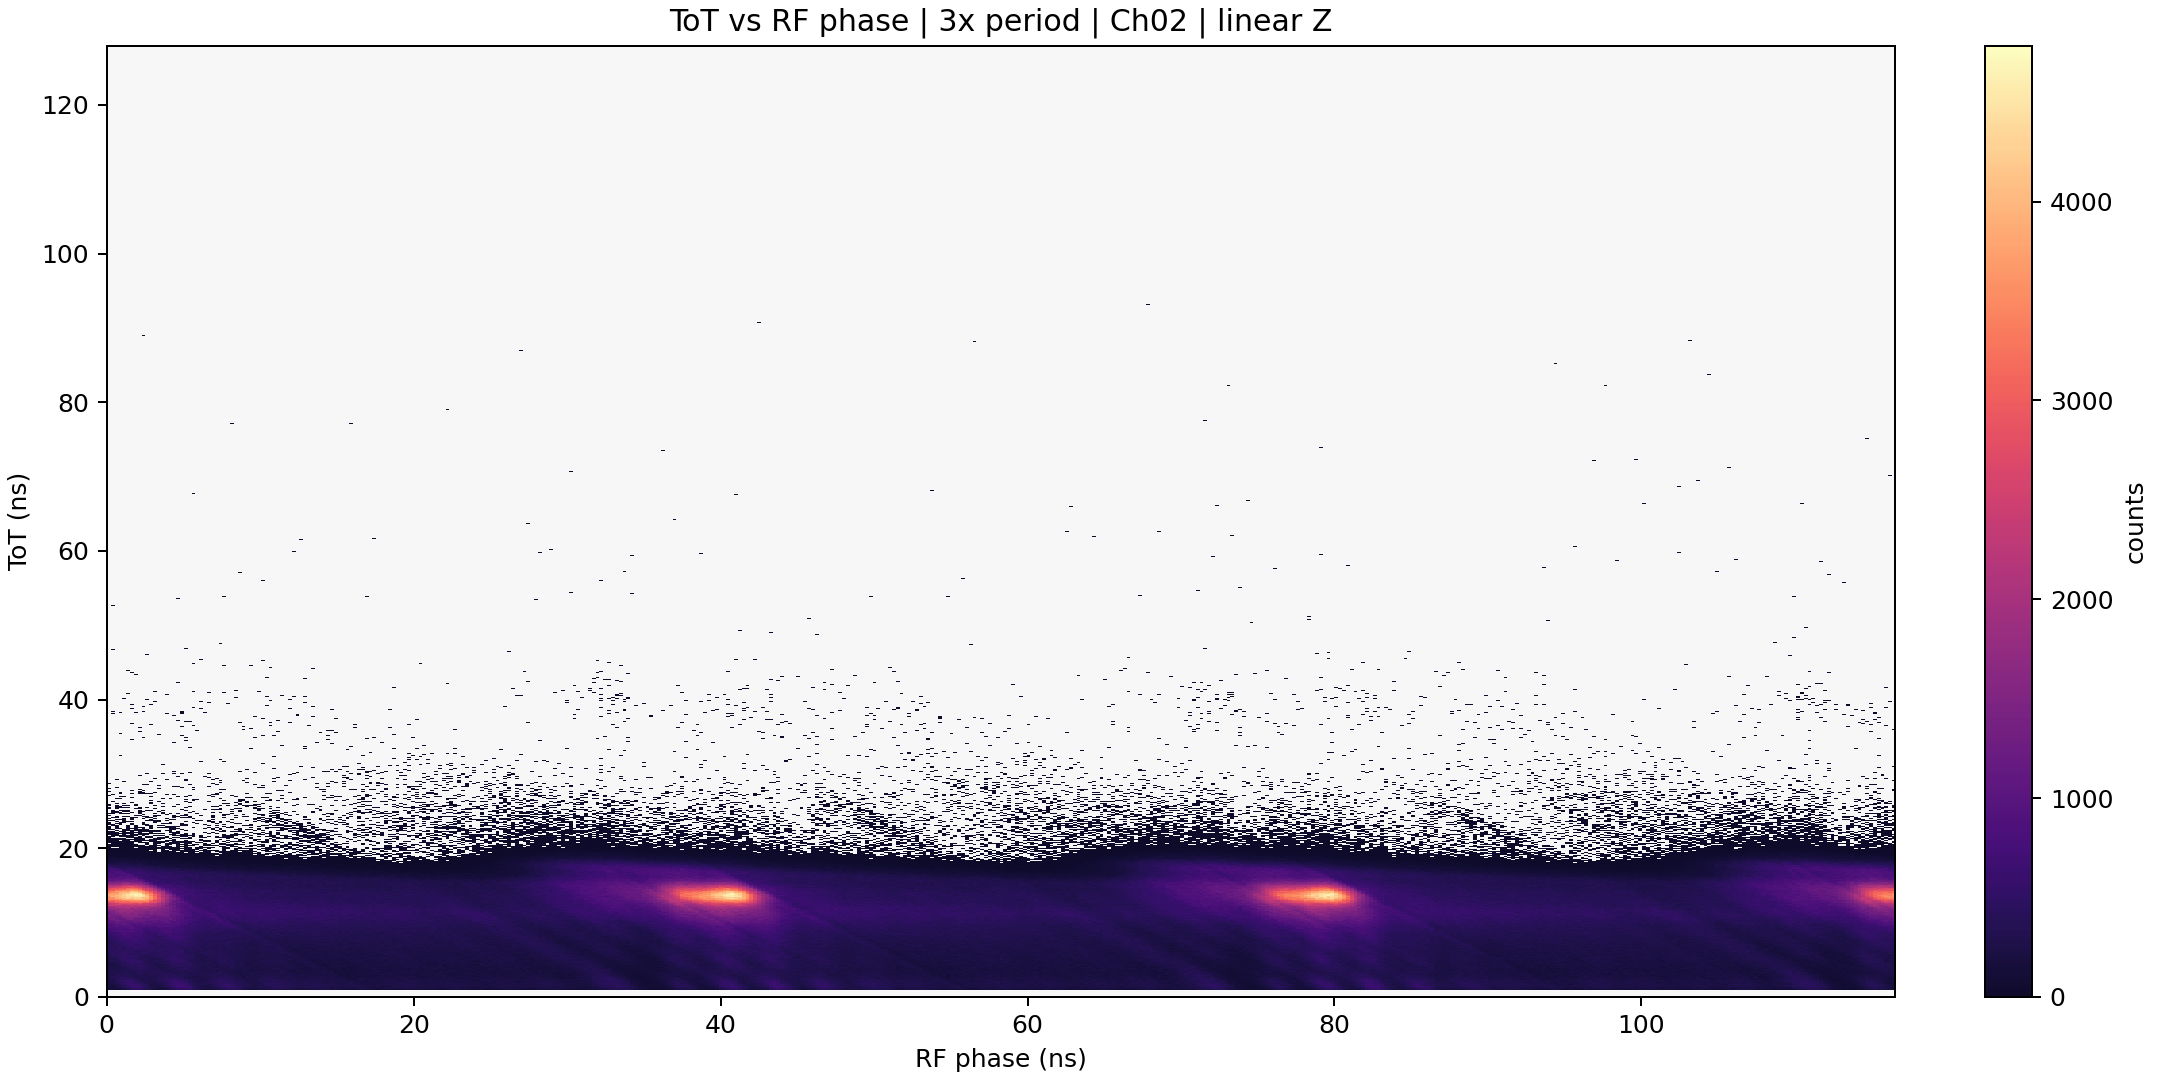
\includegraphics[width=\linewidth]{figures/phase_tot_position_scan/pos_6p6m_ch02_rf_phase_3x_vs_tot.png}
\end{minipage}
\caption{Position-scan view of NCAL channel 2 in folded RF phase and time-over-threshold. Each panel shows the same observable space over three RF periods for a different detector-face distance. The panels motivate the later gamma--neutron separation strategy: at some positions the compact prompt-like island is visibly separated from the broader neutron-dominated distribution, while in overlap regions the event content must be treated as a statistical mixture rather than by unique hit-by-hit labels. The \SI{4.0}{m} panel uses the completed \texttt{NCAL\_20us\_Pos\_4m\_0001} run.}
\label{fig:position-scan-phase-tot-panel}
\end{figure}
\end{landscape}
